\documentclass[10pt,oneside,slovak,a4paper]{article}

\usepackage[slovak]{babel}

\usepackage[IL2]{fontenc} 
\usepackage[utf8]{inputenc}
\usepackage{graphicx}
\usepackage{listings}
\usepackage{verbatim}
\usepackage{url}
\usepackage{amsfonts}
\usepackage{hyperref} 
\usepackage{cite}
\usepackage[margin=1.3in]{geometry}
\usepackage{float}

\setlength{\tabcolsep}{18pt}
\renewcommand{\arraystretch}{1.5}

\lstset{literate=%
         {á}{{\'a}}1
         {í}{{\'i}}1
         {é}{{\'e}}1
         {ý}{{\'y}}1
         {ú}{{\'u}}1
         {ó}{{\'o}}1
         {ě}{{\v{e}}}1
         {š}{{\v{s}}}1
         {č}{{\v{c}}}1
         {ľ}{{\v{l}}}1
         {ř}{{\v{r}}}1
         {ž}{{\v{z}}}1
         {ď}{{\v{d}}}1
         {ť}{{\v{t}}}1
         {ň}{{\v{n}}}1                
         {ů}{{\r{u}}}1
         {Á}{{\'A}}1
         {Í}{{\'I}}1
         {É}{{\'E}}1
         {Ý}{{\'Y}}1
         {Ú}{{\'U}}1
         {Ó}{{\'O}}1
         {Ě}{{\v{E}}}1
         {Š}{{\v{S}}}1
         {Č}{{\v{C}}}1
         {Ř}{{\v{R}}}1
         {Ž}{{\v{Z}}}1
         {Ď}{{\v{D}}}1
         {Ť}{{\v{T}}}1
         {Ň}{{\v{N}}}1                
         {Ů}{{\r{U}}}1
         {Ä}{{\"A}}1
         {Ľ}{{\v{L}}}1
         {ä}{{\"a}}1    
}

\pagestyle{headings}


\begin{document}

\begin{titlepage}
	\centering
	\par\vspace{1cm}
	{\scshape\LARGE Slovenská technická univerzita v Bratislave \par}
	{\scshape\Large Fakulta informatiky a informačných technológií\par}
	\vspace{1.5cm}
	{\large Princípy informačných systémov \par}
	{\large Dokumentácia projektu\par}
	\vspace{5cm}
	{\huge\bfseries Repozitár - digitálna knižnica\par}
	\vspace{0.5cm}
	{\Large\itshape Dávid Kubík, Martin Staňo, Veronika Včelková\par}
	\vfill
	cvičiaci\par
	RNDr. Marta \textsc{Gnipová}, Ing. Nadežda \textsc{Andrejčíková}, PhD.\par
	\vspace{1cm}
	{\large \today\par}
\end{titlepage}

\tableofcontents

\newpage


\section{Percentuálny podiel práce autov na projekte}

\vspace{1cm}

\begin{tabular}{ |p{3cm}||p{2.5cm}|p{3cm}|p{2.5cm}|}
 \hline
 \multicolumn{4}{|c|}{\textbf{Podiel práce}} \\
 \hline
 Časť projektu & Dávid Kubík & Martin Staňo & Veronika Včelková\\
 \hline
 Počiatočný návrh a identifikácia úloh & 30 & 30 &  40\\
 \hline
 Zapracovanie pripomienok z konzultácií a vytvorenie návrhu v IBM BPM & 40 & 30 &  30\\
 \hline
 Návrh formulárov & 30 & 30 &  40\\
 \hline
 Návrh použitia webových služieb & 30 & 40 &  30\\
 \hline
 Implementácia v IBM BPM & 30 & 40 &  30\\
 \hline
 Vypracovanie dokumentácie & 40 & 30 &  30\\
 
 \hline
\end{tabular}

\newpage

\section{Špecifikácia projektu: Repozitár - digitálna knižnica}

\subsection{Úvod}

Cieľom tohto projektu je definovať biznis procesy na podporu nižšie popísanej problémovej domény. Tieto biznis procesy budu navrhnuté, implementované a otestované v prostredí IBM BPM. Pri návrhu a implementácií biznis procesov sa dbalo na dodržiavanie princípov SOA (využívanie webových služieb a ich správne prepojenie).


\subsection{Špecifikácia}

Horizont H2020 určuje vedeckovýskumným pracoviskám povinnosť evidovať svoje publikované výsledky VaV v repozitári – vlastnom, konzorcionálnom, národnom. Údaje, ktoré popisujú dokument – bibliografický záznam, môže vykonávať spracovateľ, knihovník, alebo priamo vedec.

Formulár obsahuje minimálne všetky základné údaje nevyhnutné pre jednoznačnú identifikáciu daného typu dokumentu. Pri vkladaní dát sú priebežne systémom vykonávané viaceré kontroly, dôležité je, aby všetky entity boli identifikovaný perzistentným jedno-jednoznačným identifikátorom, teda aby v systéme nemohli na základe termínu reprezentujúceho dané idivídum vznikať homonymá, ale zároveň aby systém vedel k danému termínu agregovať všetky jeho synonymá, akronymy, či iné variantné formy termínov, ktoré môžu vystihovať význam tohto indivídua.

Zadané údaje sa vždy uložia do systému aj s prípadnými chybami, všetky údaje sú logované a v prípade, že neexistuje identifikátor pre dané indivídum entity, systém vytvorí nový záznam pre toto individum a pridelí mu požadovaný identifikátor a následne vo formulári prelinkuje na tento identifikátor.

Všetky vzťahy medzi entitami sú evidované na základe významu a prostredníctvom uvedených identifikátorov, teda nie odkaz na termín, ten sa generuje následne prostredníctvom daného identifikátora z príslušnej databázy modelu. 

Konečnú platnosť a správnosť údajov, môže potvrdiť až knihovník, vtedy sa všetky údaje pre iný používateľov a teda aj autorov stávajú len read/only, návrh na akúkoľvek zmenu môžu vykonať len prostredníctvom mailu, alebo poznámky k záznamu. Ak údaje vkladá spracovateľ, alebo vedecký pracovník, ostatní spoluautori ako aj konkrétny spracovateľ sú o tom informovaní , rovnako ako aj v prípade, keď knihovník potvrdí správnosť a zverejní záznam. 

Samozrejme autori určujú podmienky, pre koho bude záznam aj dokument dostupný voľne a pre ktoré skupiny na vyžiadanie, prípadne pre koho zasa úplne neviditeľný, pričom môže toto kombinovať aj s časovým určením, teda napr. pre pracovníkov oddelenia voľne dostupný pre ostatných akademických a vedecko-pedagogických pracovníkov voľne dostupný po 2 rokoch a pre ostatných viditeľný po 3 a voľne dostupný po 5 rokoch.

Navrhnite procesy, ktoré umožnia spracovať a sprístupňovať repozitár publikovaných výsledkov vedy a výskumu tak, že bude zároveň evidovať všetky vzájomné vzťahy medzi entitami použitými pre popis publikovaného výsledku VaV na základe významu.

\newpage

\subsection{Obmedzenia}
V nami implementovanom systéme sú nasledovné obmedzenia:
\begin{itemize}
\item na zobrazenie názvu, kľúčových slov a autorov bibliografického záznamu stačí, keď má vedec rank 0, to znamená, že tieto informácie sú dostupné pre všetkých prihlásených vedcov,
\item na zobrazenie abstraktu a obsahu bibliografického záznamu, musí mať vedec rank aspoň 1,
\item na zobrazenie náhľadu bibliografického záznamu, musí mať vedec rank aspoň 2,
\item na zobrazenie plného textu bibliografického záznamu musí mať vedec rank 3.
\end{itemize}

\subsection{Vypracovanie projektu}
Návrh aj implementácia nášho projektu bude realizovaná vo vývojovom prostredí IBM Business Process Designer 8.5.5. Diagram dátového modelu bude vytvorený vo webovom nástroji draw.io.


\section{Návrh, analýza a opis biznis procesov}

V tomto projekte budú analyzované a implementované nasledujúce biznis procesy súvisiace s problémovou doménou:

\begin{itemize}
\item Nahranie digitálneho objektu pre bibliografický záznam
\item Validácia digitálneho objektu
\item Nahranie bibliografického záznamu
\end{itemize}

\newpage

\subsection{Dátový model}
Vo vyššie pomenovaných biznis procesoch sme identifikovali nasledujúce entity ako aj ich atribúty a vzťahy medzi nimi. Tieto entity zároveň reprezentujú naše biznis objekty (komplexné dátové typy).

\begin{figure} [H]
\label{datamodel}
\centering
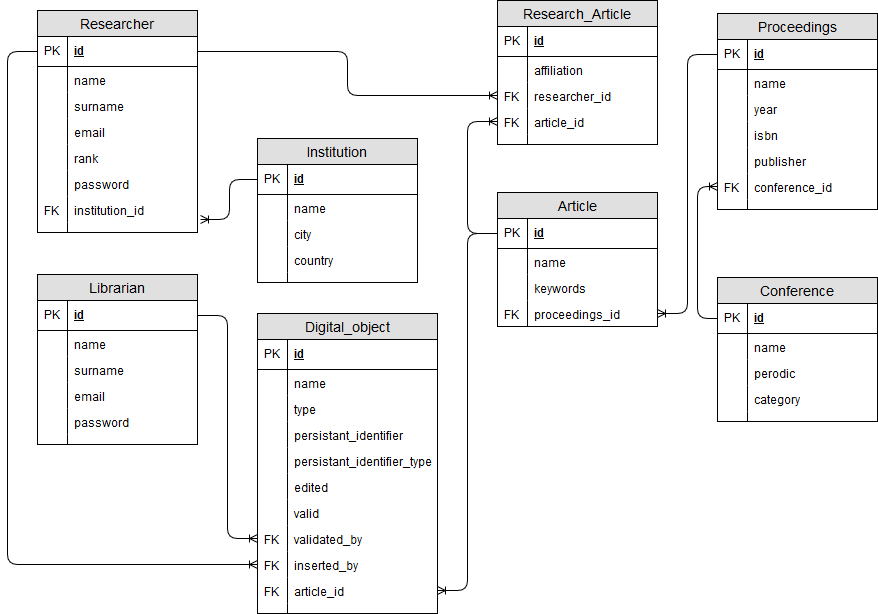
\includegraphics[scale=0.4]{datovy_model.png} 
\caption{ER diagram dátového modelu}
\end{figure}

\subsection{Biznis proces upload a bibliographic record}
V nasledujúcich podkapitolách sa bližšie pozrieme na biznis proces - nahranie bibliografického záznamu.

\subsubsection{Cieľ biznis procesu}
Cieľom tohto biznis procesu je nahranie bibliografického záznamu do konkrétneho digitálneho repozitára. Knihovník vykoná kontrolu údajov a potvrdí ich potencionálnu správnosť.

\subsubsection{Používateľské roly}
Jednotlivé kroky procesu sú rozdelené do troch plaveckých dráh.

\begin{itemize}
\item \textbf{Systém} Táto plavecká dráha obsahuje úlohy, ktoré bude vykonávať nami navrhovaný systém.
\item \textbf{Používateľ} Táto plavecká dráha obsahuje úlohy, ktoré bude vykonávať používateľ systému. Používateľom, môže byť spracovateľ, knihovník, alebo vedec.
\item \textbf{Knihovník} Táto plavecká dráha obsahuje úlohy, ktoré bude vykonávať knihovník.
\end{itemize}

\newpage

\subsubsection{Biznis objekty}
\textbf{Institution}\\
Tento biznis objekt reprezentuje vedeckovýskumné pracovisko, ktoré eviduje publikované výsledky v digitálnom repozitári. Parametre tohto biznis objektu sú nasledovné:

\begin{itemize}
\item \textbf{id:} unikátny primárny kľúč v systémovej databáze,
\item \textbf{name:} názov inštitúcie, pod ktorým je registrovaná v obchodnom registri Slovenskej republiky,
\item \textbf{city:} mesto, v ktorom má daná inštitúcia hlavné sídlo,
\item \textbf{country:} krajina, v ktorom je hlavné sídlo danej inštitúcie.
\end{itemize}

\textbf{Librarian}\\
Tento biznis objekt reprezentuje knihovníka digitálneho repozitáru, ktorý má na starosti okrem iného aj potvrdzovanie správnosti zadaných údajov digitálneho objektu bibliografického záznamu. Parametre tohto biznis objektu sú nasledovné:

\begin{itemize}
\item \textbf{id:} unikátny primárny kľúč v systémovej databáze,
\item \textbf{name:} krstné meno uvedené v rodnom liste pracovníka vedeckovýskumného ústavu,
\item \textbf{surname:} priezvisko uvedené v rodnom liste pracovníka vedeckovýskumného ústavu,
\item \textbf{email:} emailová schránka pracovníka vedeckovýskumného ústavu,
\item \textbf{password:} prístupové heslo do systému.
\end{itemize}

\textbf{Researcher}\\
Tento biznis objekt reprezentuje zamestnanca vedeckovýskumného pracoviska, ktorý svoje výsledky publikuje do digitálneho repozitára. Parametre tohto biznis objektu sú nasledovné:

\begin{itemize}
\item \textbf{id:} unikátny primárny kľúč v systémovej databáze,
\item \textbf{name:} krstné meno uvedené v rodnom liste pracovníka vedeckovýskumného ústavu,
\item \textbf{surname:} priezvisko uvedené v rodnom liste pracovníka vedeckovýskumného ústavu,
\item \textbf{email:} emailová schránka pracovníka vedeckovýskumného ústavu,
\item \textbf{rank:} úroveň pracovníka k sprístupneniu publikácií,
\item \textbf{password:} prístupové heslo do systému,
\item \textbf{institution\_id:} cudzí kľúč v systémovej databáze, ktorý sa odkazuje na konkrétnu inštitúciu.
\end{itemize}

\textbf{Research\_Article}\\
Tento biznis objekt reprezentuje prepojovaciu tabuľku v systémovej databáze medzi vedcami a publikáciami. K tomuto kroku sme pristúpili z dôvodu, aby sme vedeli korektne vyjadriť vzťah many-to-many. Parametre tohto biznis objektu sú nasledovné:

\begin{itemize}
\item \textbf{id:} unikátny primárny kľúč v systémovej databáze,
\item \textbf{affilation:} rola autora/spoluautora na danom bibliografickom zázname, napr. spoluautor, prekladateľ, ilustrátor,
\item \textbf{researcher\_id:} cudzí kľúč v systémovej databáze, ktorý sa odkazuje na autora publikovaného bibliografického záznamu v digitálnom repozitári,
\item \textbf{article\_id:} cudzí kľúč v systémovej databáze, ktorý sa odkazuje na publikovaný bibliografický záznam v digitálnom repozitári.
\end{itemize}

\textbf{Proceedings}\\
Tento biznis objekt reprezentuje zborník, ktorý vznikol ako dôsledok určitej vedeckej konferencie. Parametre tohto biznis objektu sú nasledovné:

\begin{itemize}
\item \textbf{id:} unikátny primárny kľúč v systémovej databáze,
\item \textbf{name:} názov zborníku vedeckej konferencie,
\item \textbf{year:} rok, kedy bol zborník vedeckej konferencie vydaný,
\item \textbf{isbn:} medzinárodné štandardné číslo knihy (z angl. international standard book number) pod ktorým bol zborník vedeckej konferencie publikovaný,
\item \textbf{publisher:} vydavateľ zborníku vedeckej konferencie,
\item, \textbf{conference\_id:} cudzí kľúč v systémovej databáze, ktorý sa odkazuje na vedeckú konferenciu.
\end{itemize}

\textbf{Article}\\
Tento biznis objekt reprezentuje bibliografický záznam v databáze vedeckovýskumného pracoviska. Parametre tohto biznis objektu sú nasledovné:

\begin{itemize}
\item \textbf{id:} unikátny primárny kľúč v systémovej databáze,
\item \textbf{name:} názov publikácie, pod ktorým je uvedená v databáze vedeckovýskumného pracoviska,
\item \textbf{keywords:} kľúčové slová, ktoré sa využívajú pri vyhľadaní danej publikácie v digitálnom repozitári,
\item \textbf{proceedings\_id:} cudzí kľúč v systémovej databáze, ktorý sa odkazuje na zborník vedeckej konferencie.
\end{itemize}

\textbf{Conference}\\
Tento biznis objekt reprezentuje vedeckú konferenciu. Parametre tohto biznis objektu sú nasledovné:

\begin{itemize}
\item \textbf{id:} unikátny primárny kľúč v systémovej databáze,
\item \textbf{name:} názov vedeckej konferencie,
\item \textbf{periodic:} vyjadruje pravdivostnú hodnotu periodicity vedeckej konferencie, či sa opakuje v pravidelných intervaloch,
\item \textbf{category:} oblasť výskumu vedeckej konferencie.
\end{itemize}

\textbf{Digital\_object}\\
Tento biznis objekt reprezentuje digitálny objekt uložený v digitálnom repozitári. Parametre tohto biznis objektu sú nasledovné:

\begin{itemize}
\item \textbf{id:} unikátny primárny kľúč v systémovej databáze,
\item \textbf{name:} názov digitálneho objektu v digitálnom repozitári,
\item \textbf{type:} typ digitálneho objektu, napr. abstrakt, plný text,
\item \textbf{persistent\_identifier:} perzistentný identifikátor, cez ktorý je digitálny objekt prístupná na internete,
\item \textbf{persistent\_identifier\_type:} typ perzistnentného identifikátoru, napr. doi, ark, eisp,
\item \textbf{edited:} dátum poslednej úpravy digitálneho objektu,
\item \textbf{valid:} pravdivostná hodnota vyjadrujúca, či zadané údaje v digitálnom objekte sú korektné,
\item \textbf{validated\_by:} cudzí kľúč v systémovej databáze, ktorý sa odkazuje na zamestnanca, ktorý kontroloval správnosť údajov digitálneho objektu,
\item \textbf{inserted\_by:} cudzí kľúč v systémovej databáze, ktorý sa odkazuje na zamestnanca, ktorý vložil digitálny objekt do digitálneho repozitáru,
\item \textbf{article\_id:} cudzí kľúč v systémovej databáze, ktorý sa odkazuje na bibliografický záznam, z ktorého bol digitálny objekt vytvorený.
\end{itemize}

\subsubsection{Kroky procesu upload a bibliographic record}
V tejto časti uvádzame podrobný opis krokov biznis procesu nahranie bibliografického záznamu a rozhodovacích blokov tohto biznis procesu.

\begin{itemize}
\item \textbf{Choose role - ľudská úloha}
\end{itemize}

\textbf{Rola:} Super user\\
\textbf{Výstup:} objekt \textit{chosen\_role} typu \textit{String}, ktorý vyjadruje používateľom zvolenú rolu.

Prostredníctvom grafického používateľského rozhrania používateľ zvolí pod akou rolou chce vystupovať. Ak klikne na tlačidlo \textit{Researcher}, tak bude vystupovať v systéme ako vedec. Ak klikne na tlačidlo \textit{Librarian}, tak bude vystupovať v systéme ako knihovník.

\begin{figure} [H]
\centering

\includegraphics[scale=0.7]{forms/formChooseRole.jpg} 
\caption{Formulár na výber role}
\end{figure}

\begin{itemize}
\item \textbf{Rozhodovací blok - As which role do you want to sign in?}
\end{itemize}

\textbf{Atribút rozhodovania:} \textit{chosen\_role} - zisťujeme, či je obsah daného atribútu ekvivalentný s reťazcom "librarian". Ak áno, tak biznis proces pokračuje krokom \textit{Login as librarian}. Ak nie, tak biznis proces pokračuje krokom \textit{Login as researcher}.

\begin{itemize}
\item \textbf{Login as researcher - ľudská úloha}
\end{itemize}

\textbf{Rola:} Researcher\\
\textbf{Výstup:} objekt \textit{researcher} typu \textit{Researcher} s nastavenými atribútmi:

\begin{itemize}
\item \textit{researcher.id} - unikátny primárny kľúč v systémovej databáze,
\item \textit{researcher.name} - krstné meno uvedené v rodnom liste pracovníka vedeckovýskumného ústavu,
\item \textit{researcher.surname} -  priezvisko uvedené v rodnom liste pracovníka vedeckovýskumného ústavu,
\item \textit{researcher.email} - emailová schránka pracovníka vedeckovýskumného ústavu,
\item \textit{researcher.rank} - úroveň pracovníka k sprístupneniu publikácií,
\item \textit{researcher.password} - prístupové heslo do systému,
\item \textit{researcher.institution\_id} - cudzí kľúč v systémovej databáze, ktorý sa odkazuje na konkrétnu inštitúciu.
\end{itemize}

Prostredníctvom grafického používateľského rozhrania používateľ zadá \textit{login\_id} a \textit{password}, následne po stlačení tlačidla \textit{OK}, pokračuje hlavný biznis proces.

\begin{figure} [H]
\centering
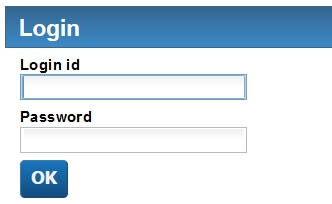
\includegraphics[scale=0.7]{forms/formLogin.jpg} 
\caption{Formulár prihlasovania vedca}
\end{figure}

\begin{itemize}
\item \textbf{Add publication or digital object
 - ľudská úloha}
\end{itemize}

\textbf{Rola:} Researcher\\
\textbf{Výstup:} objekt \textit{chosen\_action} typu \textit{String}, ktorý predstavuje voľbu používateľa, či chce pridať publikáciu alebo digitálny objekt.

Prostredníctvom grafického používateľského rozhrania používateľ zvolí kliknutím vybraného tlačidla buď \textit{Add publication} - pridanie publikácie, alebo \textit{Add digital object} - pridanie digitálneho objektu.

\begin{figure} [H]
\centering

\includegraphics[scale=0.7]{forms/formChooseAction.jpg} 
\caption{Formulár výberu akcie na pridanie publikácie alebo digitálneho objektu}
\end{figure}

\begin{itemize}
\item \textbf{Rozhodovací blok - What do you want to add?}
\end{itemize}

\textbf{Atribút rozhodovania:} \textit{researcher\_chosen\_action} - zisťujeme, či je obsah daného atribútu ekvivalentný s reťazcom "digital\_object". Ak áno, tak biznis proces pokračuje krokom \textit{Add digital object}. Ak nie, tak biznis proces pokračuje krokom \textit{Add article}.

\begin{itemize}
\item \textbf{Add article - ľudská úloha}
\end{itemize}

\textbf{Rola:} Researcher\\

Prostredníctvom grafického používateľského rozhrania používateľ zvolí vedeckú konferenciu a výber potvrdí tlačidlom \textit{Filter Proceedings}. To spôsobí, že sa vyfiltrujú v tabuľke zborníkov len tie zborníky, ktoré patria k danej vedeckej konferencii. Následne zvolí zborník vedeckej konferencie, názov článku, kľúčové slová a svoj výber potvrdí tlačidlo \textit{OK}.

\begin{figure} [H]
\centering
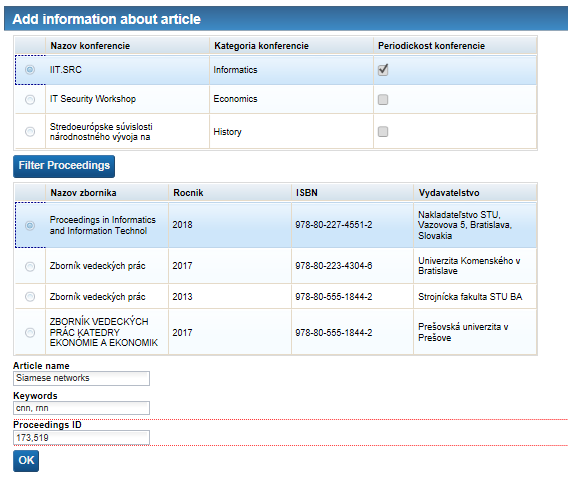
\includegraphics[scale=0.4]{forms/insert_article.png} 
\caption{Formulár pridania informácií o článku}
\end{figure}

\begin{itemize}
\item \textbf{Add coauthors - ľudská úloha}
\end{itemize}

\textbf{Rola:} Researcher\\
\textbf{Výstup:} list objektov \textit{authors\_to\_add} typu \textit{Researcher} s nastavenými atribútmi:

\begin{itemize}
\item \textit{researcher.id} - unikátny primárny kľúč v systémovej databáze,
\item \textit{researcher.name} - krstné meno uvedené v rodnom liste pracovníka vedeckovýskumného ústavu,
\item \textit{researcher.surname} -  priezvisko uvedené v rodnom liste pracovníka vedeckovýskumného ústavu,
\item \textit{researcher.email} - emailová schránka pracovníka vedeckovýskumného ústavu,
\item \textit{researcher.rank} - úroveň pracovníka k sprístupneniu publikácií,
\item \textit{researcher.password} - prístupové heslo do systému,
\item \textit{researcher.institution\_id} - cudzí kľúč v systémovej databáze, ktorý sa odkazuje na konkrétnu inštitúciu.
\end{itemize}

Tento podproces je realizovaný pomocou dvoch prepojených grafických používateľských rozhraní. Používateľ má možnosť buď pridať spolu-autora z tabuľky existujúcich vedcov alebo po kliknutí na príslušné tlačidlo môže pridať nového vedca do systému. O novom vedcovi vyplní údaje v príslušnom formulári.

\begin{figure} [H]
\centering
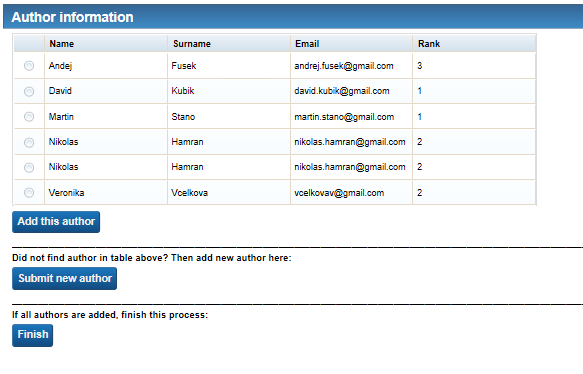
\includegraphics[scale=0.4]{forms/add_existing_coauthor.png} 
\caption{Formulár pridania existujúceho vedca ako spolu-autora}
\end{figure}

\begin{figure} [H]
\centering
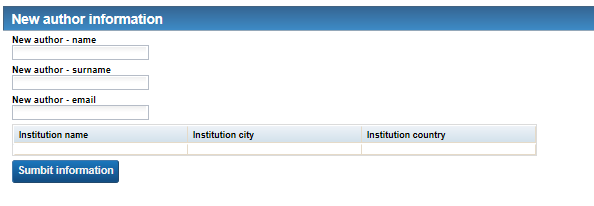
\includegraphics[scale=0.4]{forms/new_coauthor.png} 
\caption{Formulár pridania existujúceho vedca ako spolu-autora}
\end{figure}

\begin{itemize}
\item \textbf{Add digital object by researcher - ľudská úloha}
\end{itemize}

\textbf{Rola:} Researcher\\
\textbf{Vstup:} objekt \textit{logged\_researcher}\\ typu \textit{Researcher}
\textbf{Výstup:} objekt \textit{article} typu \textit{Article} s nastavenými atribútmi:

\begin{itemize}
\item \textit{researcher.id} - unikátny primárny kľúč v systémovej databáze,
\item \textit{researcher.name} - krstné meno uvedené v rodnom liste pracovníka vedeckovýskumného ústavu,
\item \textit{researcher.surname} -  priezvisko uvedené v rodnom liste pracovníka vedeckovýskumného ústavu,
\item \textit{researcher.email} - emailová schránka pracovníka vedeckovýskumného ústavu,
\item \textit{researcher.rank} - úroveň pracovníka k sprístupneniu publikácií,
\item \textit{researcher.password} - prístupové heslo do systému,
\item \textit{researcher.institution\_id} - cudzí kľúč v systémovej databáze, ktorý sa odkazuje na konkrétnu inštitúciu.
\end{itemize}

Prostredníctvom grafického používateľského rozhrania používateľ (vedec) postupne na základe konferencie \textit{(Conference)} a zberníka \textit{(Proceedings)} vyfiltruje články (\textit{Article}). Po vyplnení údajov o digitálnom objekte a kliknutí na potvrdzovacie tlačidlo sa k označenému článku priradí digitálny objekt.

\begin{figure} [H]
\centering
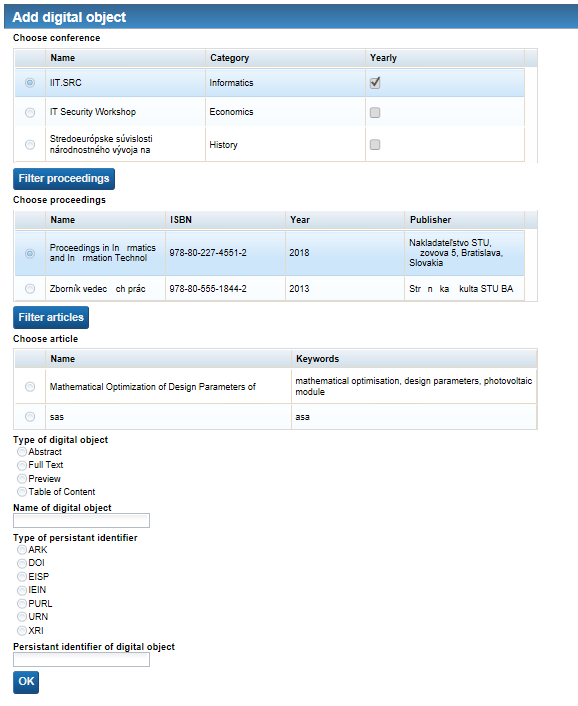
\includegraphics[scale=0.4]{forms/formAddDigital.png} 
\caption{Formulár pridania digitálneho objektu}
\end{figure}

\begin{itemize}
\item \textbf{Choice to add more digital objects by researcher
 - ľudská úloha}
\end{itemize}

\textbf{Rola:} Researcher\\
\textbf{Výstup:} objekt \textit{more\_digital\_objects} typu \textit{Boolean} je nastavený na pravdivostnú hodnotu podľa toho, či vedec chce ešte pridať ďalší digitálny objekt alebo nie.

Prostredníctvom grafického používateľského rozhrania používateľ zvolí kliknutím vybraného tlačidla buď \textit{Yes} - pridanie ďalšieho digitálneho objektu, alebo \textit{No} - ukončí sa pridávanie digitálnych objektov k článku.

\begin{figure} [H]
\centering

\includegraphics[scale=0.4]{forms/formDigitalObjects.jpg} 
\caption{Formulár pridania informácií o článku}
\end{figure}

\begin{itemize}
\item \textbf{Rozhodovací blok - Do you want to add more digital objects?}
\end{itemize}

\textbf{Atribút rozhodovania:} \textit{add\_more\_digital\_objects} - zisťujeme, či je hodnota daného atribútu ekvivalentná s pravdivostnou hodnotou false. Ak áno, tak biznis proces sa ukončí. Ak nie, tak biznis proces pokračuje krokom \textit{Add digital object by researcher}.

\begin{itemize}
\item \textbf{Validate digital object
 - ľudská úloha}
\end{itemize}

\textbf{Rola:} Librarian\\
\textbf{Vstup:} objekt \textit{librarian} typu \textit{Librarian}.

Prostredníctvom grafického používateľského rozhrania používateľ zvolí konferenciu a po kliknutí na tlačidlo \textit{Filter proceedings} vyfiltruje zborníky, ktoré patria k zvolenej konferencii. Následne používateľ vyberie konkrétny zborník a klikne na tlačidlo \textit{Filter articles}, to má za následok, že sa vyfiltrujú články pre zvolený zborník. Napokon používateľ vyberie konkrétny článok a klikne na tlačidlo \textit{Filter digital objects}. Následne si používateľ vyberie digitálny objekt a rozhodne, či sú jeho údaje korektné alebo nie.

\begin{figure} [H]
\centering
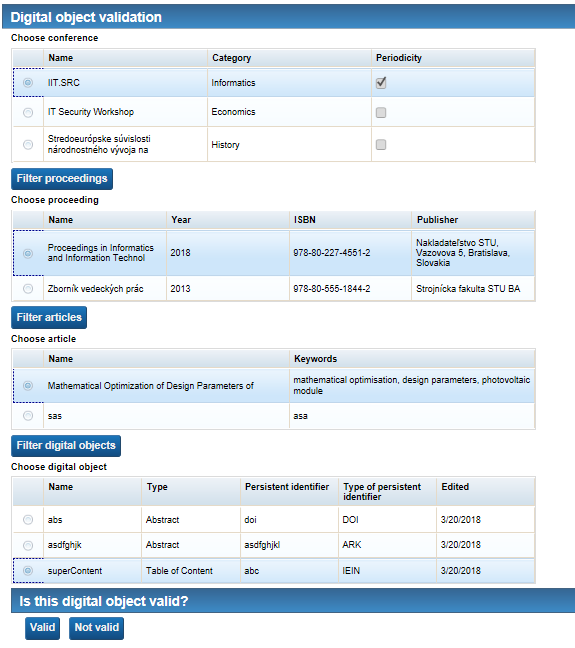
\includegraphics[scale=0.4]{forms/do_validation.png} 
\caption{Formulár validácie digitálnych objektov}
\end{figure}

\begin{itemize}
\item \textbf{Choice to add more digital objects by librarian
 - ľudská úloha}
\end{itemize}

\textbf{Rola:} Librarian\\
\textbf{Výstup:} objekt \textit{more\_digital\_objects} typu \textit{Boolean} je nastavený na pravdivostnú hodnotu podľa toho, či knihovník chce ešte pridať ďalší digitálny objekt alebo nie.

Prostredníctvom grafického používateľského rozhrania používateľ zvolí kliknutím vybraného tlačidla buď \textit{Yes} - pridanie ďalšieho digitálneho objektu, alebo \textit{No} - ukončí sa pridávanie digitálnych objektov k článku.

\begin{figure} [H]
\centering

\includegraphics[scale=0.4]{forms/formDigitalObjects.jpg} 
\caption{Formulár pre výber možnosti pridania ďalšieho digitálneho objektu}
\end{figure}

\begin{itemize}
\item \textbf{Rozhodovací blok - Do you want to add more digital objects?}
\end{itemize}

\textbf{Atribút rozhodovania:} \textit{add\_more\_digital\_objects} - zisťujeme, či je hodnota daného atribútu ekvivalentná s pravdivostnou hodnotou false. Ak áno, tak biznis proces sa ukončí. Ak nie, tak biznis proces pokračuje krokom \textit{Add digital object by librarian}.


%Martinova cast

\begin{itemize}
\item \textbf{Login as Librarian}
\end{itemize}

\textbf{Rola:} Librarian\\
\textbf{Výstup:} objekt \textit{logged\_librarian} typu \textit{Librarian}, ktorý vyjadruje prihláseného knihovníka.

Prostredníctvom grafického používateľského rozhrania používateľ (knihovník) zadá svoje prihlasovacie údaje, ktoré sa v danom podprocese overia (prebehne autentifikácia). V prípade nesprávnych údajov za zobrazí chybová hláška a tok procesu prihlásenia sa vráti na začiatok procesu. V prípade správnych prihlasovacích údajov pokračuje biznis proces ďalšou aktivitou.

\begin{figure} [H]
\centering
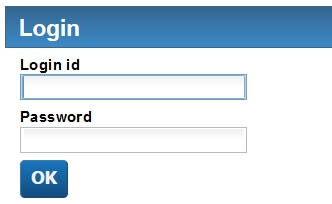
\includegraphics[scale=0.7]{forms/formLogin.jpg} 
\caption{Formulár prihlasovania vedca}
\end{figure}

\begin{itemize}
\item \textbf{Validate or Add Digital Object}
\end{itemize}

\textbf{Rola:} Librarian\\
\textbf{Výstup:} objekt \textit{chosen\_action} typu \textit{String}, ktorý vyjadruje akciu zvolenú používateľom (knihovníkom).

\begin{figure} [H]
\centering

\includegraphics[scale=0.7]{forms/formChooseActionLib.png} 
\caption{Formulár na vybratie akcie, či validovať alebo pridať digitálny objekt}
\end{figure}

Prostredníctvom grafického používateľského rozhrania používateľ (knihovník) na základe kliknutia na jedno z dvoch tlačidiel zvolí akciu ktorú si želá ďalej v rámci biznis procesu vykonať.

\begin{itemize}
\item \textbf{Add Digital Object by Librarian}
\end{itemize}

\textbf{Rola:} Librarian\\
\textbf{Vstup:} objekt \textit{librarian} typu \textit{Librarian},  ktorý predstavuje prihláseného knihovníka
\textbf{Výstup:} objekt \textit{article} typu \textit{Article}, článok ku ktorému bol pridaný digitálny objekt. Článok je výstup procesu pretože, po tomto procese nasleduje proces \textit{Send Notifications by Librarian}, ktorý každému spoluatorovi článku ku ktorému bol pridaný digitálny objekt pošle notifikáciu.

Prostredníctvom grafického používateľského rozhrania používateľ (knihovník) postupne na základe konferencie \textit{(Conference)} a zberníka \textit{(Proceedings)} vyfiltruje články (\textit{Article}). Po vyplnení údajov o digitálnom objekte a kliknutí na potvrdzovacie tlačidlo sa k označenému článku priradí digitálny objekt.

\begin{figure} [H]
\centering
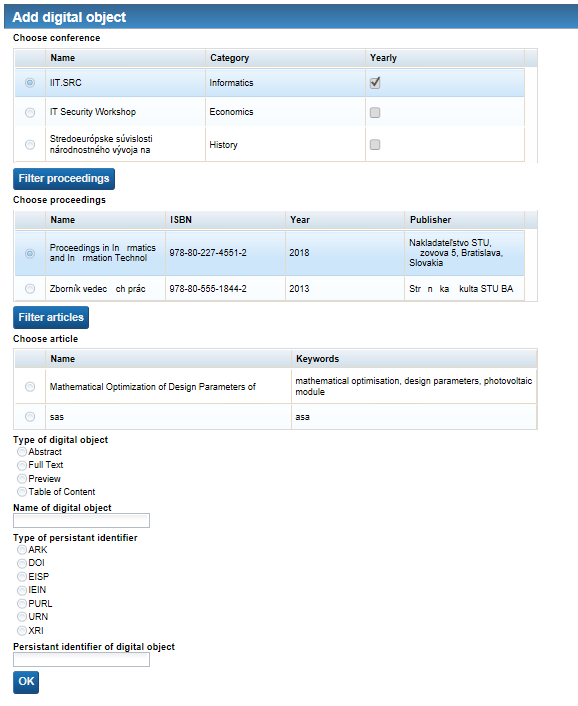
\includegraphics[scale=0.4]{forms/formAddDigital.png} 
\caption{Formulár pridania digitálneho objektu}
\end{figure}

\section{Implementácia systémových úloh}

\begin{itemize}
\item \textbf{Send notification by librarian - systémová úloha}
\end{itemize}

\textbf{Rola:} System\\
\textbf{Vstup:} objekt \textit{article} typu \textit{Article}.

\begin{itemize}
\item \textbf{article.id:} unikátny primárny kľúč v systémovej databáze,
\item \textbf{article.name:} názov publikácie, pod ktorým je uvedená v databáze vedeckovýskumného pracoviska,
\item \textbf{article.keywords:} kľúčové slová, ktoré sa využívajú pri vyhľadaní danej publikácie v digitálnom repozitári,
\item \textbf{article.proceedings\_id:} cudzí kľúč v systémovej databáze, ktorý sa odkazuje na zborník vedeckej konferencie.
\end{itemize}

Systém získa všetky entity prepojovacej tabuľky Article-Researcher. Vyfiltruje tie záznamy, ktoré zodpovedajú konkrétnemu článku. Pre každý vyfiltrovaný záznam získa vedca a tomu pošle notifikáciu. Vedec môže byť notifikovaný email-om, alebo prostredníctvo SMS správy, alebo obidvoma spôsobmi.

\begin{figure} [H]
\centering
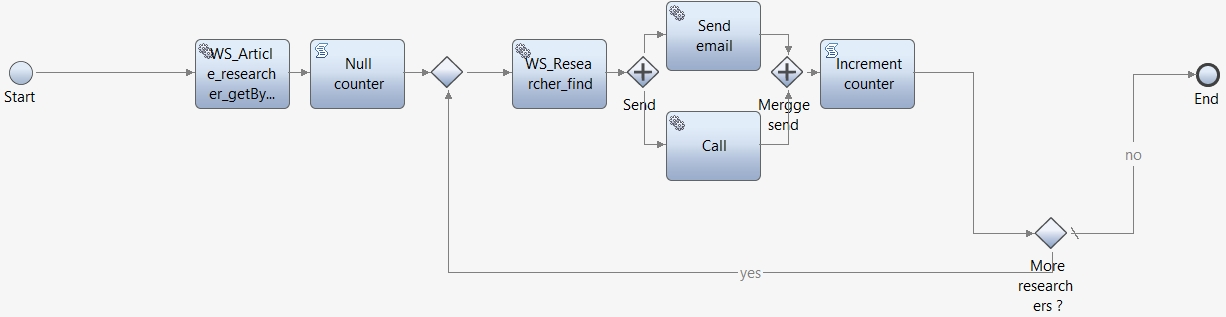
\includegraphics[scale=0.4]{diagrams/diagNotification.jpg} 
\caption{Diagram podprocesu poslania notifikácií}
\end{figure}

\begin{itemize}
\item \textbf{Send notification by researcher - systémová úloha}
\end{itemize}

\textbf{Rola:} System\\
\textbf{Vstup:} objekt \textit{article} typu \textit{Article}.

\begin{itemize}
\item \textbf{article.id:} unikátny primárny kľúč v systémovej databáze,
\item \textbf{article.name:} názov publikácie, pod ktorým je uvedená v databáze vedeckovýskumného pracoviska,
\item \textbf{article.keywords:} kľúčové slová, ktoré sa využívajú pri vyhľadaní danej publikácie v digitálnom repozitári,
\item \textbf{article.proceedings\_id:} cudzí kľúč v systémovej databáze, ktorý sa odkazuje na zborník vedeckej konferencie.
\end{itemize}

Systém získa všetky entity prepojovacej tabuľky Article-Researcher. Vyfiltruje tie záznamy, ktoré zodpovedajú konkrétnemu článku. Pre každý vyfiltrovaný záznam získa vedca a tomu pošle notifikáciu. Vedec môže byť notifikovaný email-om, alebo prostredníctvo SMS správy, alebo obidvoma spôsobmi.

\begin{figure} [H]
\centering
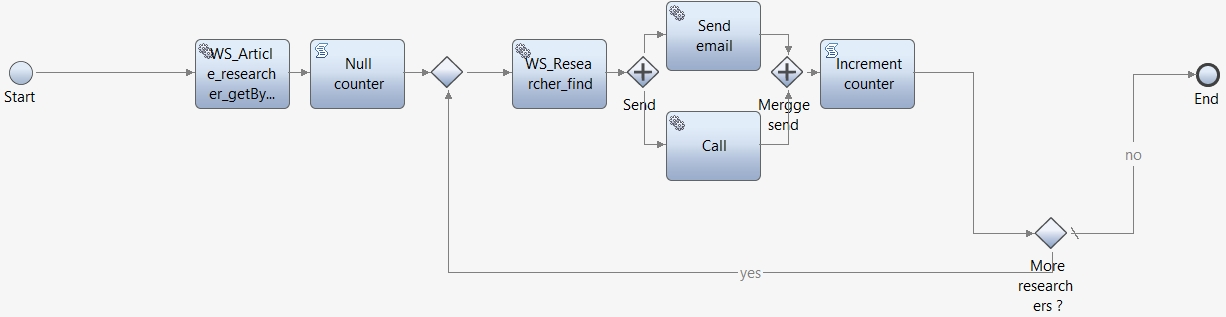
\includegraphics[scale=0.4]{diagrams/diagNotification.jpg} 
\caption{Diagram podprocesu poslania notifikácií}
\end{figure}







\subsection{Webová služba: Získanie vedeckej publikácie}
\textbf{Názov služby:} WS\_Article\_find
\textbf{Metóda služby:} getById
\textbf{Vstupy:}
	\begin{itemize}
		\item \textit{id} - ID vedeckej publikácie
	\end{itemize}
\textbf{Výstupy:}
	\begin{itemize}
		\item \textit{article} - objekt typu Article
	\end{itemize}
	
\subsection{Webová služba: Získanie všetkých vedeckých publikácií}
\textbf{Názov služby:}  WS\_Article\_findAll
\textbf{Metóda služby:} getAll
\textbf{Výstupy:}
	\begin{itemize}
		\item \textit{articles} - list objektov typu Article
	\end{itemize}
	
\subsection{Webová služba: Získanie vedeckých publikácií na základe atribútu}
\textbf{Názov služby:} WS\_Article\_getByAttribute
\textbf{Metóda služby:} getByAttributeValue
\textbf{Vstupy:}
	\begin{itemize}
		\item \textit{attributes\_name} - názov atribútu
		\item \textit{attributes\_value} - hodnota atribútu
		\item \textit{listOf.Integer()} - zoznam ID vedeckých publikácií, z ktorých sa má vyhľadávať
	\end{itemize}
\textbf{Výstupy:}
	\begin{itemize}
		\item \textit{articles} - list objektov typu Article
	\end{itemize}
	
\subsection{Webová služba: Vloženie vedeckej publikácie}
\textbf{Názov služby:} WS\_Article\_insert
\textbf{Metóda služby:} insert
\textbf{Vstupy:}
	\begin{itemize}
		\item \textit{team\_id} - ID tímu, slúži na autentifikáciu webovej služby
		\item \textit{team\_password} - heslo, slúži na autentifikáciu webovej služby
		\item \textit{Article} - objekt typu Article s vyplnenými údajmi
	\end{itemize}
\textbf{Výstupy:}
	\begin{itemize}
		\item \textit{id} - ID novo vytvorenej vedeckej publikácie
	\end{itemize}
	
\subsection{Webová služba: Získanie všetkých vedeckých konferencií}
\textbf{Názov služby:} WS\_Conference\_findAll
\textbf{Metóda služby:} getAll
\textbf{Výstupy:}
	\begin{itemize}
		\item \textit{conferences} - list objektov typu Conference
	\end{itemize}
	
\subsection{Webová služba: Vloženie vedeckej konferencie}
\textbf{Názov služby:} WS\_Conference\_insert
\textbf{Metóda služby:} insert
\textbf{Vstupy:}
	\begin{itemize}
		\item \textit{team\_id} - ID tímu, slúži na autentifikáciu webovej služby
		\item \textit{team\_password} - heslo, slúži na autentifikáciu webovej služby
		\item \textit{Conference} - objekt typu Conference s vyplnenými údajmi
	\end{itemize}
\textbf{Výstupy:}
	\begin{itemize}
		\item \textit{id} - ID novo vytvorenej vedeckej konferencie
	\end{itemize}
	
\subsection{Webová služba: Získanie všetkých digitálnych objektov}
\textbf{Názov služby:} WS\_Digital\_object\_findAll
\textbf{Metóda služby:} getAll
\textbf{Výstupy:}
	\begin{itemize}
		\item \textit{digital\_objects} - list objektov typu Digital\_object
	\end{itemize}
	
\subsection{Webová služba: Vloženie digitálneho objektu}
\textbf{Názov služby:} WS\_Digital\_object\_insert
\textbf{Metóda služby:} insert
\textbf{Vstupy:}
	\begin{itemize}
		\item \textit{team\_id} - ID tímu, slúži na autentifikáciu webovej služby
		\item \textit{team\_password} - heslo, slúži na autentifikáciu webovej služby
		\item \textit{digital\_object} - objekt typu Digital\_object s vyplnenými údajmi
	\end{itemize}
\textbf{Výstupy:}
	\begin{itemize}
		\item \textit{id} - ID novo vytvoreného digitálneho objektu
	\end{itemize}
	
\subsection{Webová služba: Získanie zborníka podľa vedeckej konferencie}
\textbf{Názov služby:} WS\_Get\_proceedings\_by\_conference
\textbf{Metóda služby:} getByAttributeValue
\textbf{Vstupy:}
	\begin{itemize}
		\item \textit{attributes\_name} - názov atribútu
		\item \textit{attributes\_value} - hodnota atribútu
		\item \textit{listOf.Integer()} - zoznam ID zborníkov, z ktorých sa má vyhľadávať
	\end{itemize}
\textbf{Výstupy:}
	\begin{itemize}
		\item \textit{proceedings} - list objektov typu Proceeding
	\end{itemize}
	
\subsection{Webová služba: Získanie všetkých inštitúcií}
\textbf{Názov služby:} WS\_Institution\_findAll
\textbf{Metóda služby:} getAll
\textbf{Výstupy:}
	\begin{itemize}
		\item \textit{institutions} - list objektov typu Institution
	\end{itemize}
	
\subsection{Webová služba: Vloženie inštitúcie}
\textbf{Názov služby:} WS\_Institution\_insert
\textbf{Metóda služby:} insert
\textbf{Vstupy:}
	\begin{itemize}
		\item \textit{team\_id} - ID tímu, slúži na autentifikáciu webovej služby
		\item \textit{team\_password} - heslo, slúži na autentifikáciu webovej služby
		\item \textit{institution} - objekt typu Institution s vyplnenými údajmi
	\end{itemize}
\textbf{Výstupy:}
	\begin{itemize}
		\item \textit{id} - ID novo vytvorenej inštitúcie
	\end{itemize}
	
\subsection{Webová služba: Získanie knihovníka}
\textbf{Názov služby:} WS\_Librarian\_find
\textbf{Metóda služby:} getById
\textbf{Vstupy:}
	\begin{itemize}
		\item \textit{id} - ID knihovníka
	\end{itemize}
\textbf{Výstupy:}
	\begin{itemize}
		\item \textit{librarian} - objekt typu Librarian
	\end{itemize}
	
\subsection{Webová služba: Získanie všetkých knihovníkov}
\textbf{Názov služby:} WS\_Librarian\_findAll
\textbf{Metóda služby:} getAll
\textbf{Výstupy:}
	\begin{itemize}
		\item \textit{librarians} - list objektov typu Librarian
	\end{itemize}
	
\subsection{Webová služba: Vloženie knihovníka}
\textbf{Názov služby:} WS\_Librarian\_insert
\textbf{Metóda služby:} insert
\textbf{Vstupy:}
	\begin{itemize}
		\item \textit{team\_id} - ID tímu, slúži na autentifikáciu webovej služby
		\item \textit{team\_password} - heslo, slúži na autentifikáciu webovej služby
		\item \textit{librarian} - objekt typu Librarian s vyplnenými údajmi
	\end{itemize}
\textbf{Výstupy:}
	\begin{itemize}
		\item \textit{id} - ID novo vytvoreného knihovníka
	\end{itemize}
	
\subsection{Webová služba: }
\textbf{Názov služby:} WS\_
\textbf{Metóda služby:} 
\textbf{Vstupy:}
	\begin{itemize}
		\item \textit{} - 
	\end{itemize}
\textbf{Výstupy:}
	\begin{itemize}
		\item \textit{} - 
	\end{itemize}
	
\subsection{Webová služba: }
\textbf{Názov služby:} WS\_
\textbf{Metóda služby:} 
\textbf{Vstupy:}
	\begin{itemize}
		\item \textit{} - 
	\end{itemize}
\textbf{Výstupy:}
	\begin{itemize}
		\item \textit{} - 
	\end{itemize}
	
\subsection{Webová služba: }
\textbf{Názov služby:} WS\_
\textbf{Metóda služby:} 
\textbf{Vstupy:}
	\begin{itemize}
		\item \textit{} - 
	\end{itemize}
\textbf{Výstupy:}
	\begin{itemize}
		\item \textit{} - 
	\end{itemize}
	
\subsection{Webová služba: }
\textbf{Názov služby:} WS\_
\textbf{Metóda služby:} 
\textbf{Vstupy:}
	\begin{itemize}
		\item \textit{} - 
	\end{itemize}
\textbf{Výstupy:}
	\begin{itemize}
		\item \textit{} - 
	\end{itemize}
	
	
	
	



\newpage

\section{Zhrnutie}
Táto práca je výsledkom analýzy získanej témy pre zadávanie bibliografických dokumentov a digitálnych objektov v systéme digitálneho repozitáru. Spracované sú biznis procesy, ktoré boli identifikované na základe zadania a následných konzultácií. Podobným spôsobom boli identifikované roly používateľov systému, ktoré majú rôzne práva. 

Základom práce bolo navrhnúť proces predstavujúci najpodstatnejšiu časť systému, a to pridanie článku, so všetkými atribútmi, ktoré ho definujú a pridanie a validovanie digitálneho objektu článku - príkladom je náhľad alebo abstrakt konkrétneho bibliografického dokumentu. Spolu s tým boli definované jeho podprocesy spolu s formulármi, ktoré sú základom k implementovaniu funkcionality systému. Formuláre boli navrhnuté tak, aby boli čo najviac prehľadné, intuitívne a aby nimi boli zabezpečené správne entitno-relačné prepojenia v databáze, kde sme sa snažili vyhnúť zadávaniu id objektu, na ktorý má byť vytváraný objekt mapovaný. Riešením bolo ponúknuť používateľovi na výber z dostupných možností alebo ponúknutie vytvorenia objektu a jeho následné mapovanie.

Kvôli komplexnosti problémov vyplývajúcim zo zadania sa však používatelia prihlasujú práve pod spomínaným id a heslom, kde id poskytuje jednoznačný identifikátor, ktorý bolo vhodné použiť pri identifikácii.

V návrhu sú zahrnuté webové služby, najmä na notifikáciu používateľov ale i iné, súvisiace s databázou objektov a manipuláciou s nimi.

Návrhom sme sa snažili pokryť zadanie čo najlepšie nám to dané prostriedky a webové služby dovoľovali.

\section{Report prác členov tímu}
\subsection{Dávid Kubík}
K vypracovaniu analýzy zadanej témy sme sa podielali v prvotných krokoch spoločne, kde sa definovali roly používateľov systému a entitno-relačný model. Potom sme prácu spracovávali paralelne v IBM Designer, pričom sme stále medzi sebou konzultovali nápady. To zahŕňalo definovanie webových služieb a najmä tvorbu formulárov. Jedným z ďalších bodov, na ktorom som sa výrazne podielal, bola tvorba dokumentácie k našej analýze, opísanie procesu, podprocesov, biznis objektov a celkovo fungovaniu návrhu.
\subsection{Martin Staňo}
K tomu, aby sme boli schopní vypracovať zadanie spoločne bez zbytočných nedorozumení sme zvolili prvotný brainstorming, kde sa definovali základné myšlienky, roly, procesy. Všetko sa konzultovalo až do bodu, kedy bola rozdelená ďalšia práca na projekte. V IBM som následne definoval základné služby, ktoré sme potrebovali k ďalšej práce a následne som pracoval na formulároch pre podprocesy a aj na samotných podprocesoch. Pri dokumentácii som prispel opisom vybraných podprocesov a pridaním screenshotov formulárov, ktoré v práci opisujeme.
\subsection{Veronika Včelková}
Náplň mojej práce spočívala v spoločnom prvotnom identifikovaní biznis objektov, ich prepojení a atribútov, rolí, ktoré vystupujú v systéme a náčrtu hlavného biznis procesu. Následne som sa zamerala na implementáciu v IBM Process Designer, kde som mala priradené webové služby vyplývajúce z objektov z nášho dátového modelu a následne priradené podprocesy definujúce hlavný biznis proces.



\end{document}